\chapter{Konzept und Architektur}
\label{chap:concept&architecture}
Dieses Kapitel erläutert den konzeptionellen Aufbau der erweiterten Check-API. Dafür werden die Anforderungen aus Kapitel \ref{chap:requirements} in die Zielarchitektur, den Ablauf einer Anfrage und in die Sicherheitsmaßnamen übersetzt.

\section{Überblick über die Zielarchitektur}
Die Zielarchitektur baut dabei auf der bereits bestehenden isolierten Check-API, sowie den bestehenden Systemen, wie der Haupt-API, Frontend und Datenbank auf.
Die Haupt-API ist für die Verwaltung aller Anfragen, sowie der Zusammensetzung notwendiger Daten zuständig. Für die Prüfung des Nutzercodes ruft sie die Check-API auf und übergibt die notwendigen Informationen, wie die öffentlichen Tests, Nutzercode und die neu eingeplanten verstecken Tests.

Die Check-API übernimmt, separiert vom restlichen System, den Prüfdienst, die Verarbeitung der Einreichung und liefert ein Ergebnis an die Haupt-API zurück. Die Weiterentwicklung im Rahmen dieser Bachelorarbeit setzt primär hier an und erweitert das System um eine sichere Hidden-Test-Verarbeitung, einer Überprüfung auf bösartige Codeabschnitte und eine aussagekräftige Ergebnisrückgabe. 

Abbildung \ref{fig:Konzept-Architektur Chapter4} zeigt den konzeptionellen Aufbau der Zielarchitektur. Die Haupt-API sammelt die Daten und leitet sie an die Check-API weiter. Damit bleibt die Haupt-API für die Verwaltung und die Check-API ist weiterhin für die Prüfung zuständig.
\begin{figure}[htbp]
	\centering
	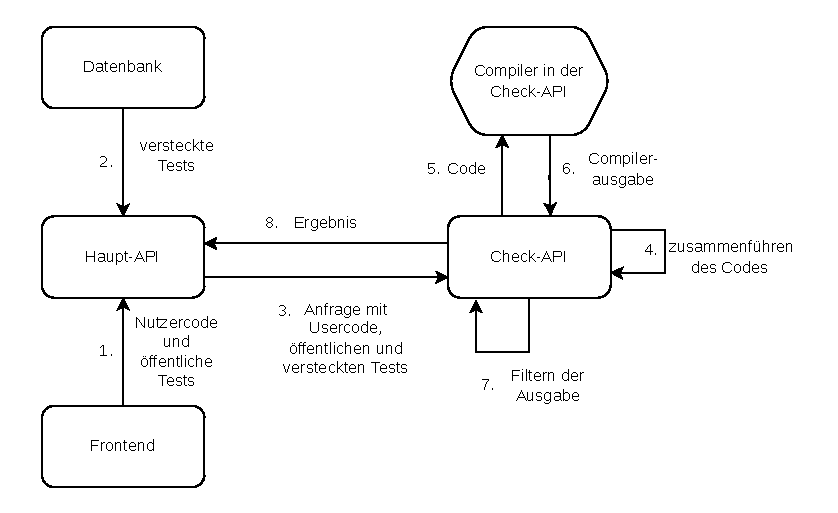
\includegraphics[width=0.8\textwidth]{diagrams/Konzept-Architektur Chapter4.pdf}
	\caption{Konzept-Architektur}
	\label{fig:Konzept-Architektur Chapter4}
\end{figure}

\section{Verarbeitungsablauf einer Einreichung}
Zu beginn der Verarbeitung schickt die Haupt-API eine Anfrage an die Check-API, in dieser Anfrage sind bereits die öffentlichen, versteckten Tests und der Nutzercode enthalten. Die Check-API nimmt diese Daten entgegen verarbeitet diese und vereint sie für eine einzige Ausführung. So können, wie bisher, die öffentlichen Tests, Nutzercode und mit der Änderung auch die versteckten Tests gemeinsam compiliert und ausgeführt werden. Das ist wichtig, damit beide Testsysteme mit den entsprechenden Daten arbeiten können, ohne das der gleiche Nutzercode zwei mal ausgeführt werden muss. Tritt bei der Kompilierung oder der Ausführung ein Fehler auf, wird die Codeausführung terminiert, die Compiler Ergebnisse von der Check-API überprüft und relevante Informationen zurück an die Haupt-API übergeben. Zeitgleich mit der Ausführung des Nutzercodes in der Check-API, überwacht die Check-API wie lange eine Ausführung dauert. Dauert diese zu lange, wird die Ausführung beendet und die Check-API Antwortet der Haupt-API mit einer entsprechenden Nachricht.

\section{Konzept zur Hidden-Test-Integration}
Hidden oder zu deutsch versteckte Tests haben den Nutzen, zu prüfen, ob der Nutzer die Aufgabe auf die vorgesehene Art und Weise löst. Versteckte Tests gehen dabei über öffentliche Tests hinaus, sie sind dem Nutzer verborgen, sodass er diese nicht gezielt umgehen kann. Das Problem mit öffentlichen Tests ist, das sie vom Nutzer gesehen werden. Genau das ist auch der Sinn von öffentlichen Tests. Dadurch das der Nutzer sie allerdings sehen kann, kann der Nutzer den Test auch einfach umgehen, wie schon in der Analyse des Altsystems und Problemstellung \ref{section:analyseDesAltsystemsUndProblemstellung} erklärt. Versteckte Tests umgehen dies, da der Nutzer nicht sieht, was diese Tests genau prüfen.
Damit die versteckten Tests versteckt bleiben, werden diese nicht wie die öffentlichen Tests beim Aufrufen einer Aufgabe ans Frontend übergeben, sondern werden erst hinzugezogen, sobald der Nutzer seine Aufgabe abgibt. In diesem Moment wird der Nutzercode zusammen mit den öffentlichen Tests und weiteren Informationen an die Haupt-API geschickt. Die Haupt-API kann mit den zusätzlichen Informationen die versteckten Tests in der Datenbank anfragen und so gemeinsam alle drei Bestandteile an die Check-API überreichen. So wird sicher gestellt, das die genauen Testdaten der versteckten Tests nicht im Frontend einsehbar sind. Des weiteren muss sichergestellt werden, das bei der Ausführung des Codes in der Check-API im Falle eines Anschlagen eines versteckten Tests, die Ausgaben des Stacktraces abgefangen werden. Die Ausgaben des Stacktraces beinhalten genaue Details darüber, warum der Test fehlgeschlagen ist. Würden diese Informationen an den Nutzer gelangen, könnte dieser mithilfe der Informationen die Tests präzise umgehen. Das würde den Nutzen von versteckten Tests nichtig machen. Anstelle des Stacktraces soll dem Nutzer eine generische Nachricht übergeben werden, mit welcher der Nutzer versteht was falsch ist, ohne genau zu wissen, die er den Test umgehen kann.

\section{Konzept zur isolierten Codeausführung}
Zur Isolierung gehören mehrere kritische Bausteine. Angefangen mit einer Abkapselung des Compilers vom restlichen System. Das wurde erreicht durch das Aufbauen eines neuen Services, der Check-API. Diese Abkapselung ist kritisch, da sie dafür sorgt, das im Falle eines bösartigen Nutzercodes nicht das gesamte System, sonder nur dieser Service beeinträchtigt wird. Fällt der Service aus, kann das restliche System noch unbeeinträchtigt weiter arbeiten. Ausschließlich dieser Service kann nicht mehr erreicht werden. Natürlich ist ein Ausfall eines Services dennoch problematisch. Würde ein Ausgefallener Service keinen Unterschied machen, wäre dieser Service schlicht weg irrelevant. Die Check-API hat allerdings einen der wichtigsten Aufgaben in diesem System. Wie ein möglicher Ausfall des Services unproblematischer gemacht werden kann, wird in Kapitel \ref{chap:implementierung} Implementierung genauer erläutert.
Ein weiterer Schritt der Isolierung ist, den Service robust gegen die Ursachen eines Ausfalls zu machen. Die größte Schwäche der Check-API ist, das bösartiger Code sie ausschalten kann. Daher muss der auszuführende Nutzercode auf kritische Inhalte untersucht werden. Sollte solch ein kritischer Inhalt entdeckt werden, darf die Ausführung nicht stattfinden. Die Anfrage muss unterbrochen werden und mit einer entsprechenden Nachricht geantwortet werden.
Zusätzlich ist in der Isolierung die Abgrenzung von Ressourcen relevant. Im Kontext der Check-API bedeutet das, zum einen, das die Check-API selbst, keinerlei Zugriff auf Dateien oder Informationen der anderen Services haben darf. Andere Services nutzen kritische Daten, wie Zugangsinformationen für die Datenbank oder API-Schlüssel externer Services. Teilt sich die Check-API ein nicht isoliertes System mit solch anderen Services, kann sich bösartiger Nutzercode Zugriff zu genau diesen Informationen verschaffen. Wie diese Isolierung im Detail erreicht wird, wird im Kapitel \ref{chap:implementierung} Implementierung genauer aufgeschlüsselt.

\section{Konzept zur Ergebnis- und Fehlerbehandlung}
Fehlerbehandlung ist für eine Programmier-Lernplattform mit eins der entscheidendsten Elemente für die Gewährleistung  eines Erfolgreichen Lernfortschrittes. Ohne ein klares Ergebnis weiß ein Nutzer nicht, ob sein Code richtig oder falsch war. Aber hier hört es nicht auf. Der Nutzer muss auch wissen, warum etwas nicht erfolgreich war. Hier muss unterschieden werden, welche Fehler es geben kann, und wie mit diesen Umgegangen werden muss. In CodeTask müssen 6 Fälle behandelt werden, um sicherzustellen, das der Nutzer das best mögliche Ergebnis mitgeteilt bekommt. Angefangen mit bösartigem Nutzercode, welcher noch vor der Compilierung abgefangen werden muss um eine Ausführung zu verhindern, was anderen Falls zu kritischen Fehlern sorgen kann. In solch einem Fall muss mit einer Aussage geantwortet werden, welche dem Nutzer nicht mitteilt, was exakt im Code diesen Fehler ausgelöst hat, sondern lediglich das die Ausführung verboten ist. Der zweite Fall tritt auf, sollte der Nutzercode Fehler beinhalten, welche dafür sorgen, das der Compiler den Code nicht ordnungsgemäß compilieren kann. In diesem Fall kann der von dem Compiler selbst bereitgestellten Fehler dem Nutzer übergeben werden.  Der dritte Fall tritt auf, sollte es bei der Ausführung, nach der Compilierung zu Fehlern kommen. Hier kann ebenfalls der Stacktrace direkt an den Nutzer gehen ohne vorherige Filterung. Fall vier und fünf entstehen, wenn der öffentliche oder der versteckte Test anschlägt. Bei einem öffentlichen Test kann ebenfalls der Stacktrace ausgegeben werden. Bei versteckten Tests muss das System die Ausgabe abfangen, um die Geheimhaltung des Tests zu gewährleisten. Stattdessen muss auch hier eine generische Fehlermeldung dem Nutzer geantwortet werden. Der letzte Fall ist die Zeitüberschreitung, sollte der Nutzercode zu lange ausgeführt werden. In diesem Fall wird die Ausführung nach einer vordefinierten Zeit abgebrochen. Darüber muss der Nutzer allerdings Informiert werden. Auch hier kommt eine generische Antwort zum Einsatz, da es unterschiedliche Gründe geben kann, warum der Nutzercode so lange in der Ausführung braucht.


